% !TeX program = pdfLaTeX
\documentclass[12pt]{article}
\usepackage{amsmath}
\usepackage{graphicx,psfrag,epsf}
\usepackage{enumerate}
\usepackage{natbib}
\usepackage{textcomp}
\usepackage[hyphens]{url} % not crucial - just used below for the URL
\usepackage{hyperref}
\providecommand{\tightlist}{%
  \setlength{\itemsep}{0pt}\setlength{\parskip}{0pt}}

%\pdfminorversion=4
% NOTE: To produce blinded version, replace "0" with "1" below.
\newcommand{\blind}{0}

% DON'T change margins - should be 1 inch all around.
\addtolength{\oddsidemargin}{-.5in}%
\addtolength{\evensidemargin}{-.5in}%
\addtolength{\textwidth}{1in}%
\addtolength{\textheight}{1.3in}%
\addtolength{\topmargin}{-.8in}%

%% load any required packages here




\begin{document}


\def\spacingset#1{\renewcommand{\baselinestretch}%
{#1}\small\normalsize} \spacingset{1}


%%%%%%%%%%%%%%%%%%%%%%%%%%%%%%%%%%%%%%%%%%%%%%%%%%%%%%%%%%%%%%%%%%%%%%%%%%%%%%

\if0\blind
{
  \title{\bf Calendar-based graphics for visualizing people's daily schedules}

  \author{
        Earo Wang \\
    Department of Econometrics and Business Statistics, Monash University\\
     and \\     Dianne Cook \\
    Department of Econometrics and Business Statistics, Monash University\\
     and \\     Rob J Hyndman \\
    Department of Econometrics and Business Statistics, Monash University\\
      }
  \maketitle
} \fi

\if1\blind
{
  \bigskip
  \bigskip
  \bigskip
  \begin{center}
    {\LARGE\bf Calendar-based graphics for visualizing people's daily schedules}
  \end{center}
  \medskip
} \fi

\bigskip
\begin{abstract}
Calendars are broadly used in society to display temporal information and events. This paper describes a new R package with functionality to organize and display temporal data, collected on sub-daily resolution, into a calendar layout. The function \texttt{frame\_calendar} uses linear algebra on the date variable to restructure data into a format lending itself to calendar layouts. The user can apply the grammar of graphics to create plots inside each calendar cell, and thus the displays synchronize neatly with \textbf{ggplot2} graphics. The motivating application is studying pedestrian behavior in Melbourne, Australia, based on counts which are captured at hourly intervals by sensors scattered around the city. Faceting by the usual features such as day and month, was insufficient to examine the behavior. Making displays on a monthly calendar format helps to understand pedestrian patterns relative to events such as work days, weekends, holidays, and special events. The layout algorithm has several format options and variations. It is implemented in the R package \textbf{sugrrants}.
\end{abstract}

\noindent%
{\it Keywords:} data visualization, statistical graphics, time series, grammar of graphics, R
\vfill

\newpage
\spacingset{1.45} % DON'T change the spacing!

\hypertarget{introduction}{%
\section{Introduction}\label{introduction}}

We develop a method for organizing and visualizing temporal data, collected at sub-daily intervals, into a calendar layout. The calendar format is created using linear algebra, giving a restructuring of the data, that can then be integrated into a data pipeline. The core component of the pipeline is to visualise the resulting data using the grammar of graphics \citep{wilkinson2006grammar, wickham2009ggplot2}, as used in \textbf{ggplot2} \citep{R-ggplot2}, which defines plots as a functional mapping from data points to graphical primitives. The data restructuring approach is consistent with the tidy data principles available in the \textbf{tidyverse} \citep{R-tidyverse} suite. The methods are implemented in a new R package called \textbf{sugrrants} \citep{R-sugrrants}.

The purpose of the calendar-based visualization is to provide insights into people's daily schedules relative to events such as work days, weekends, holidays, and special events. This work was originally motivated by studying foot traffic in the city of Melbourne, Australia \citep{ped}. There have been 43 sensors installed that count pedestrians every hour across the inner-city area until the end of 2016 (Figure \ref{fig:ped-map}). The data set can shed light on people's daily rhythms, and assist the city administration and local businesses with event planning and operational management. A routine examination of the data would involve constructing conventional time series plots to catch a glimpse of temporal patterns. The faceted plots in Figure \ref{fig:time-series-plot} give an overall picture of the foot traffic at three different sensors over 2016. Further faceting by day of the week (Figure \ref{fig:facet-time}) provides a better glimpse of the daily and sub-daily pedestrian patterns. Faceting generates small multiples \citep{tufte1983visual} or trellis displays \citep{becker_visual_1996}, where different subsets of the same data are displayed based on conditioning variables, allowing for comparison across subsets. A series of graphics can be further grouped together to create multiple yet different data views, that forms ensemble graphics \citep{unwin_ensemble_2018}.

However, the conventional displays of time series data conceal patterns relative to special events (such as public holidays and recurring cultural/sport events), which may be worth noting to viewers.

\begin{figure}

{\centering 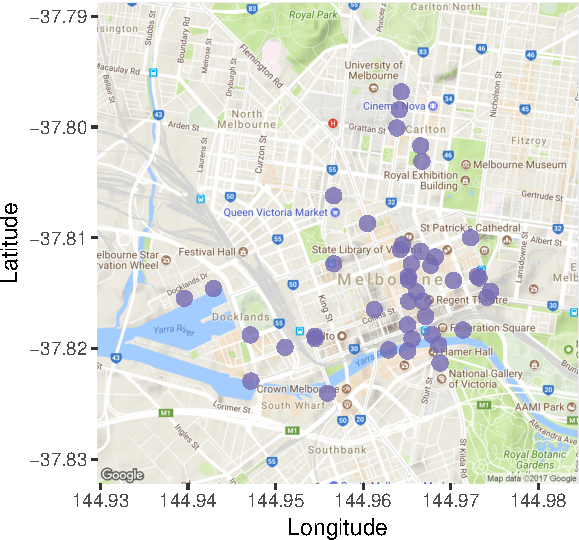
\includegraphics[width=0.7\linewidth]{figure/ped-map-1} 

}

\caption{Map of the Melbourne city area with dots indicating sensor locations. These three highlighted sensors will be inspected in the paper: (1) the State Library---a public library, (2) Flagstaff Station---a train station, closed on non-work days, (3) Birrarung Marr---an outdoor park hosting many cultural and sports events.}\label{fig:ped-map}
\end{figure}



\begin{figure}

{\centering 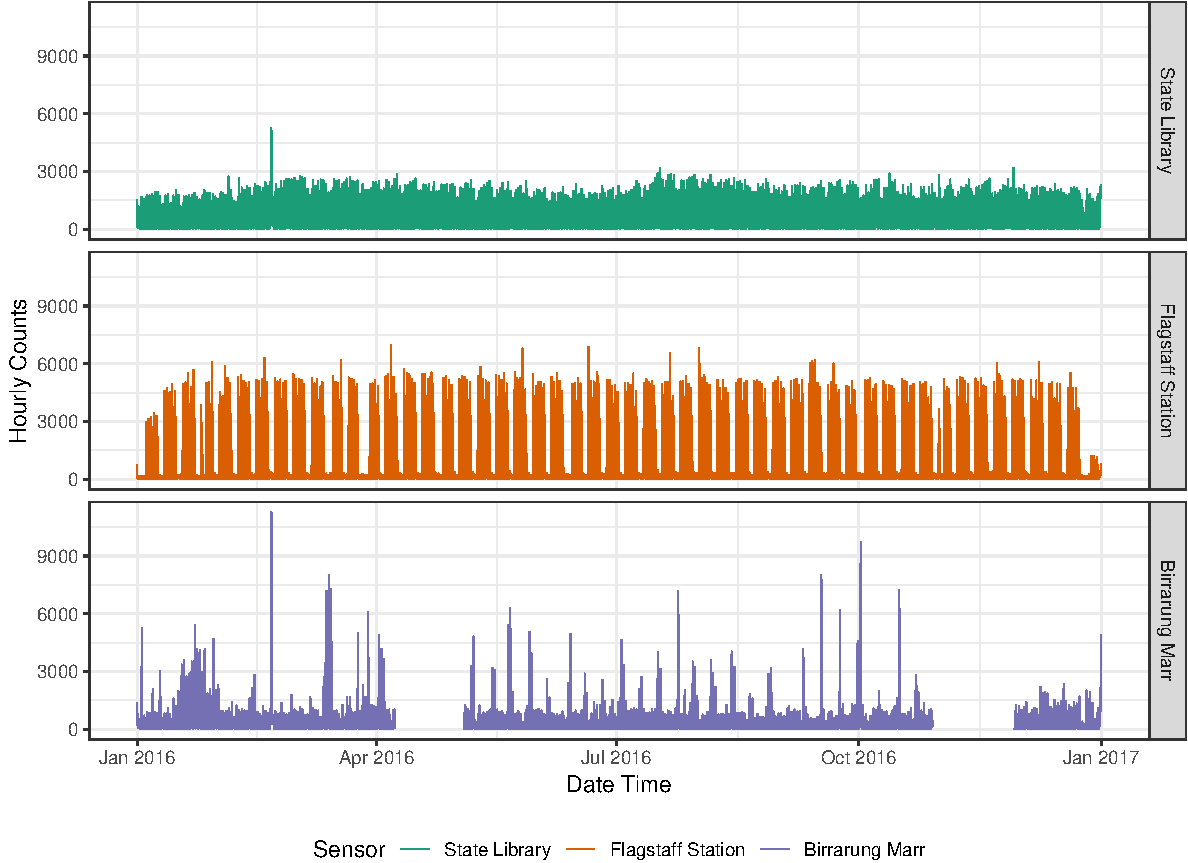
\includegraphics[width=\textwidth]{figure/time-series-plot-1} 

}

\caption{Time series plots showing the number of pedestrians in 2016 measured at three different sensors in the city of Melbourne. Colored by the sensors, small multiples of lines show that the foot traffic varies from one sensor to another in terms of both time and number. A spike occurred at the State Library, caused by the annual White Night event on 20th of February. A relatively persistent pattern repeats from one week to another at Flagstaff Station. Birrarung Marr looks rather noisy and spiky, with a couple of chunks of missing records.}\label{fig:time-series-plot}
\end{figure}



\begin{figure}

{\centering 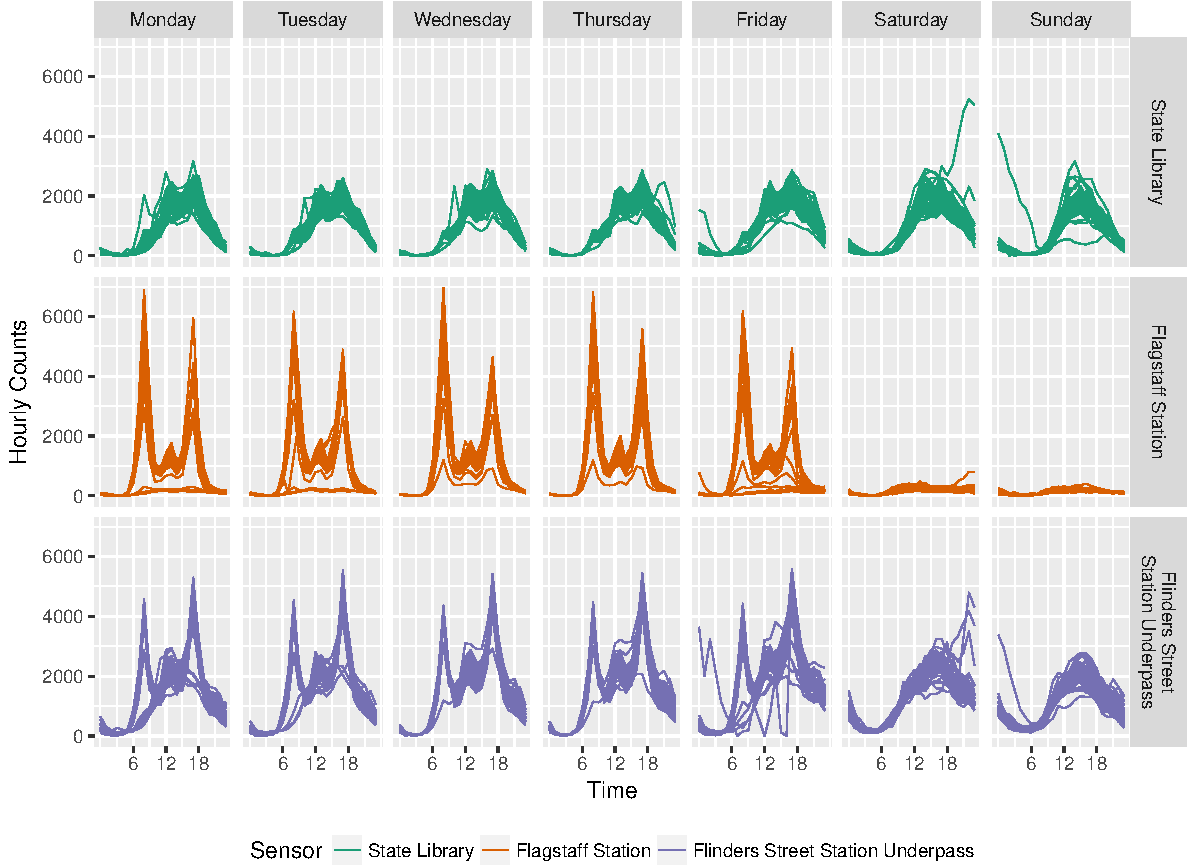
\includegraphics[width=\textwidth]{figure/facet-time-1} 

}

\caption{Hourly pedestrian counts for 2016 faceted by sensors and days of the week using lines. It primarily features two types of seasons---time of day and day of week---across all the sensors. Apparently other factors have influence over the number of pedestrians, which cannot be captured by the faceted plots, such as the overnight White Night traffic on Saturday at the State Library and a variety of events at Birrarung Marr.}\label{fig:facet-time}
\end{figure}



The work is inspired by \citet{Wickham2012glyph}, which uses linear algebra to display spatio-temporal data as glyphs on maps. It is also related to recent work by \citet{R-geofacet} which provides methods in the \textbf{geofacet} R package to arrange data plots into a grid, while preserving the geographical position. Both of these show data in a spatial context.

In contrast, calendar-based graphics unpack the temporal variable, at different resolutions, to digest multiple seasonalities and special events. There is some existing work in this area. For example, \citet{VanWijkCluster1999} developed a calendar view of the heatmap to represent the number of employees in the work place over a year, where colors indicate different clusters derived from the days. It contrasts week days and weekends, highlights public holidays, and presents other known seasonal variation such as school vacations, all of which have influence over the turn-outs in the office. Alongside \citet{Jones-heatmap}, \citet{R-TimeProjection}, \citet{R-ggTimeSeries}, and \citet{R-ggcal} implemented some variants of calendar-based heatmaps as in R packages: \textbf{TimeProjection}, \textbf{ggTimeSeries}, and \textbf{ggcal} respectively. However, these techniques are limited to color-encoding graphics and are unable to use time scales smaller than a day. Time of day, which serves as one of the most important aspects in explaining substantial variations arising from the pedestrian sensor data, will be neglected through daily aggregation. Additionally, if simply using colored blocks rather than curves, it may become perceptually difficult to estimate the shape positions and changes, although using curves comes with the cost of more display capacity \citep{cleveland1984graphical, lam2007overview}.

We propose a new algorithm to go beyond the calendar-based heatmap. The approach is developed with three conditions in mind: (1) to display time-of-day variation in addition to longer temporal components such as day-of-week and day-of-year; (2) to incorporate line graphs and other types of glyphs into the graphical toolkit for the calendar layout; (3) to enable patterns related to special events more easily pop-up to viewers. The proposed algorithm has been implemented in the \texttt{frame\_calendar} function in the \textbf{sugrrants} package using R.

The remainder of the paper is organized as follows. Section \ref{sec:algorithm} demonstrates the construction of the calendar layout in depth. Section \ref{sec:transformation} describes the algorithms of data transformation. Section \ref{sec:opt} lists and describes the options that come with the \texttt{frame\_calendar} function. Section \ref{sec:variations} presents some variations of its usage. The calendar layout is a type of faceting, and Section \ref{sec:facet-calendar} develops this into a fully-fledged faceting method with formal labels and axes. Graphical analyses of sub-daily people's activities are illustrated with a case study in Section \ref{sec:case}. Section \ref{sec:discussion} discusses the limitations of calendar displays and possible new directions.

\hypertarget{sec:algorithm}{%
\section{Creating a calendar display}\label{sec:algorithm}}

\hypertarget{sec:transformation}{%
\subsection{Data transformation}\label{sec:transformation}}

The algorithm of transforming data for constructing a calendar plot uses linear algebra, similar to that used in the glyph map displays for spatio-temporal data \citep{Wickham2012glyph}. To make a year long calendar requires cells for days, embedded in blocks corresponding to months, organized into a grid layout for a year. Each month conforms to a layout of 5 rows and 7 columns, where the top left is Monday of week 1, and the bottom right is Sunday of week 5 by default. These cells provide a micro canvas on which to plot the data. The first day of the month could be any of Monday--Sunday, which is determined by the year of the calendar. Months are of different lengths, ranging from 28 to 31 days, and some months could extend over six weeks but for these months we intentionally wrap the last few days up to the top row of the block for the purpose of compact displays. The notation for creating these cells is as follows:

\begin{itemize}
\tightlist
\item
  \(k = 1, \dots , 7\) is the day of the week that is the first day of the month.
\item
  \(d = 28, 29, 30\) or \(31\) representing the number of days in any month.
\item
  \((i, j)\) is the grid position where \(1 \le i \le 5\) is week within the month, \(1 \le j \le 7\), is day of the week.
\item
  \(g = k, \dots,(k+d)\) indexes the day in the month, inside the 35 possible cells.
\end{itemize}

The grid position for any day in the month is given by

\begin{equation}
  \begin{aligned}
  i &= \lceil (g \text{ mod } 35) / 7\rceil, \\
  j &= g \text{ mod } 7.
  \end{aligned}
  \label{eq:grid}
\end{equation}

Figure \ref{fig:month-diagram} illustrates this \((i, j)\) layout for a month where \(k=5\).

\begin{figure}

{\centering 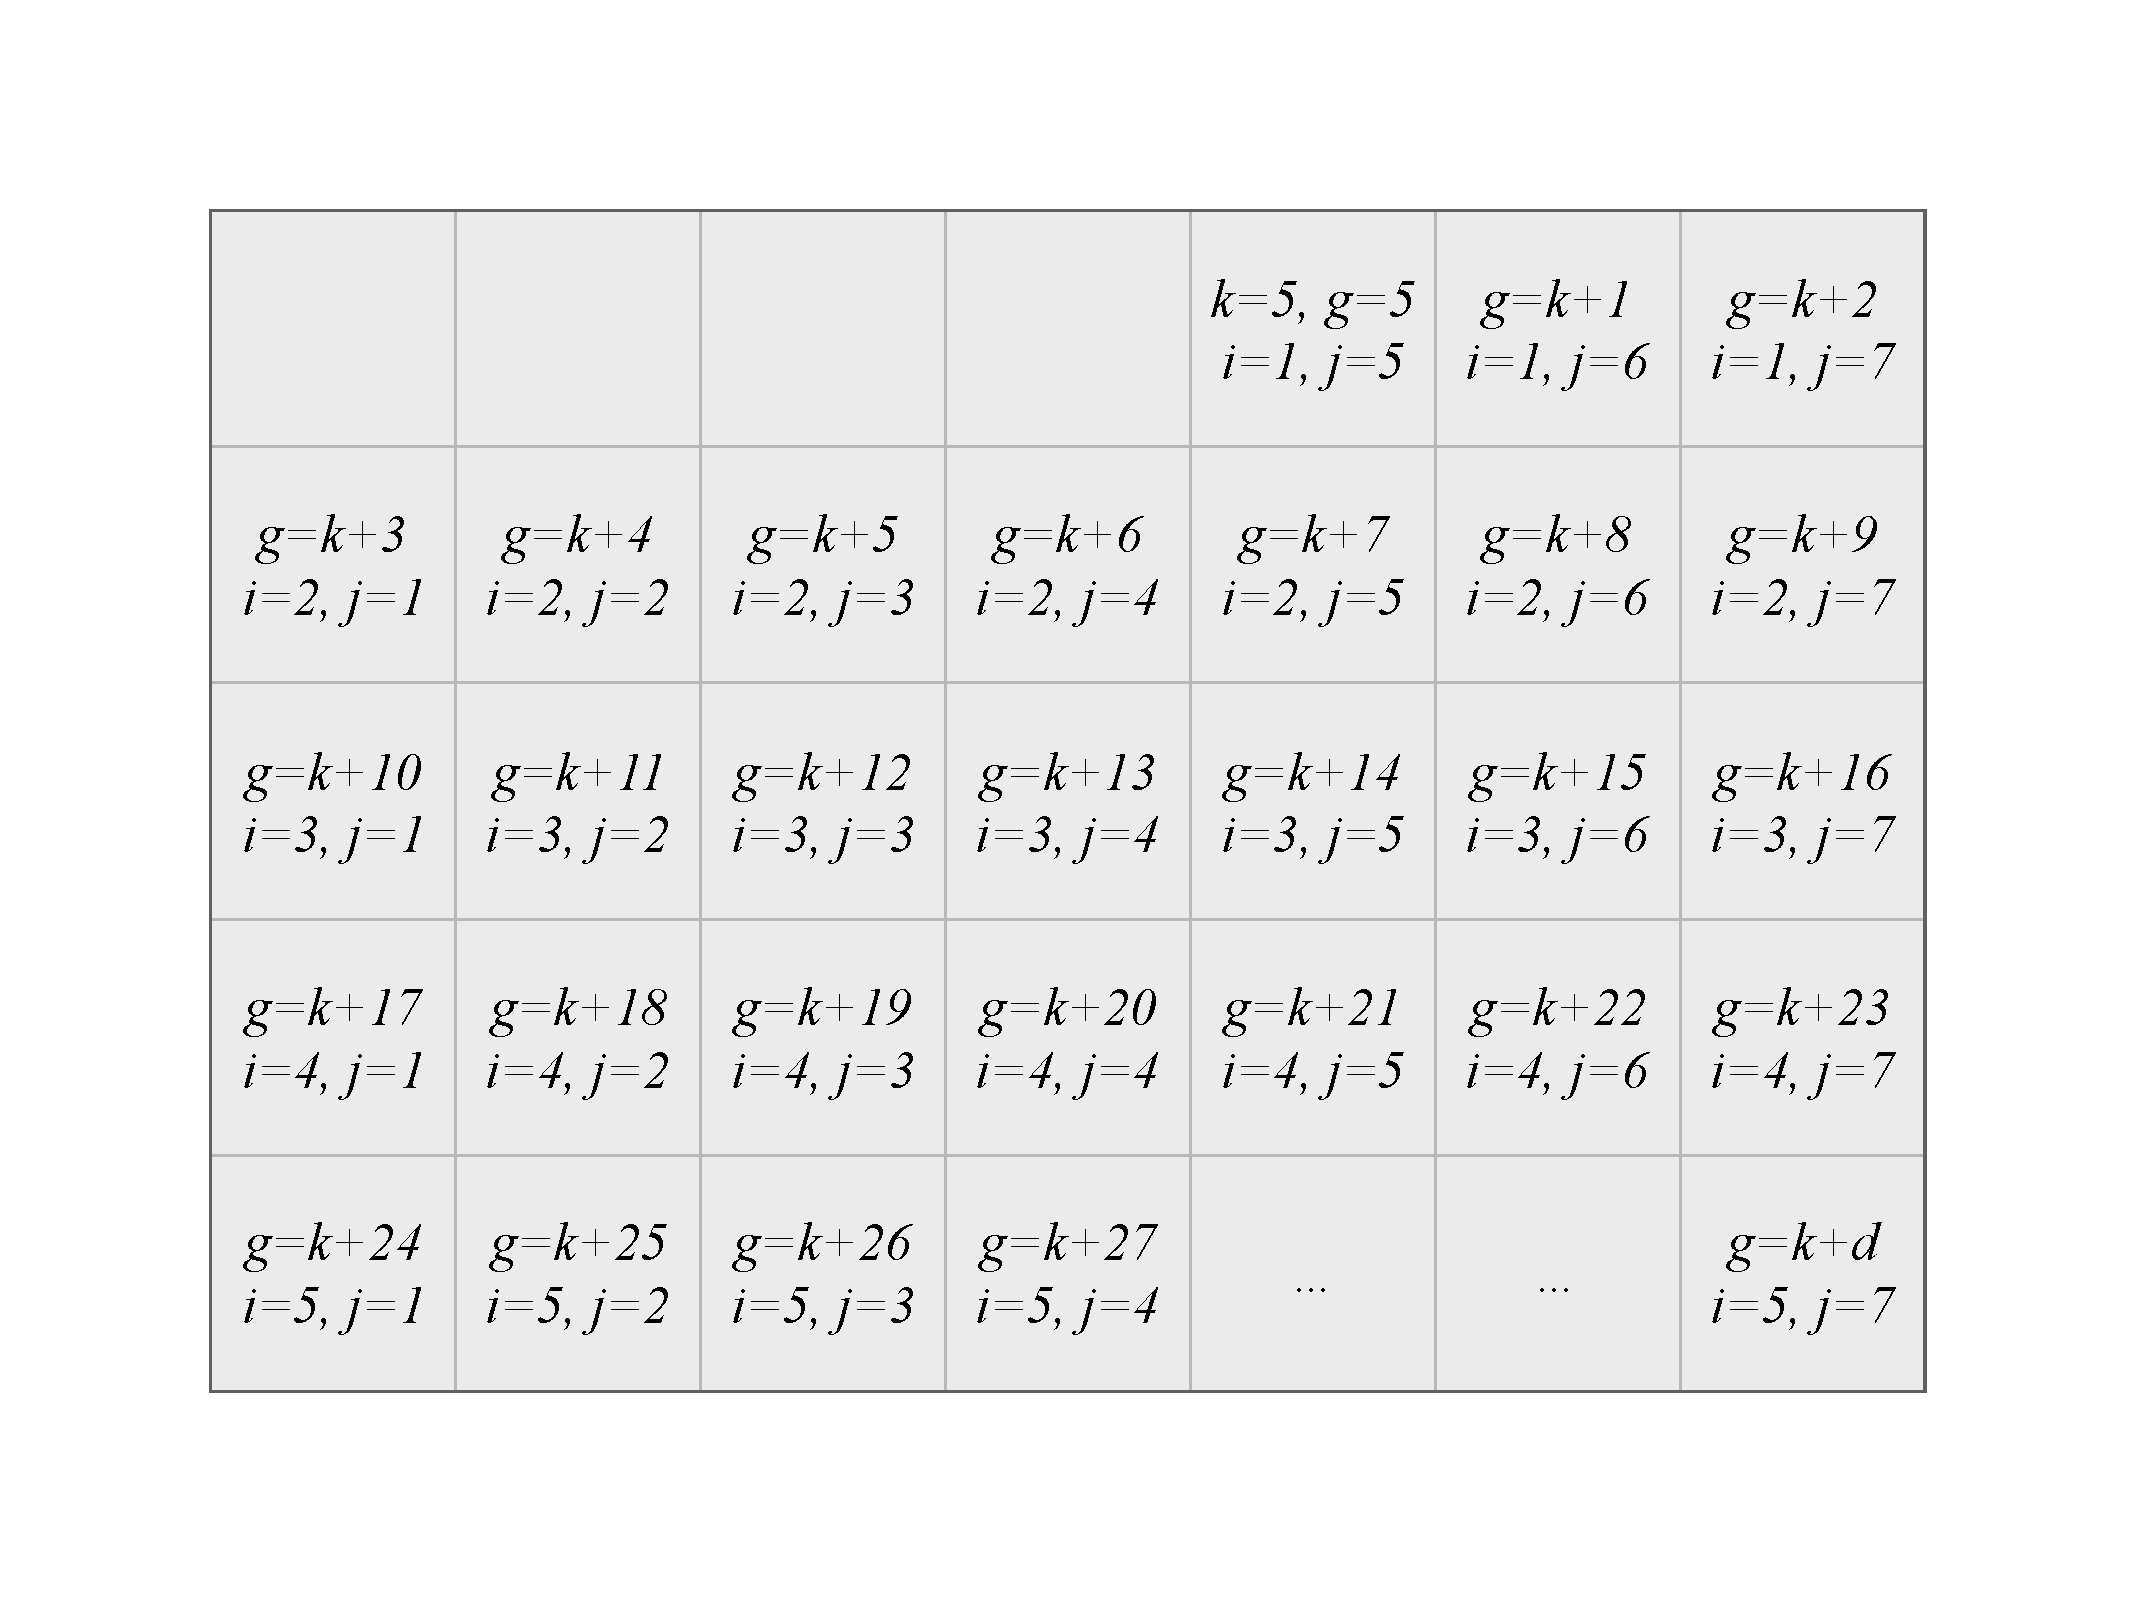
\includegraphics[width=360pt,height=250pt]{img/month} 

}

\caption{Illustration of the indexing layout for cells in a month, where \(k\) is day of the week, \(g\) is day of the month, \((i, j)\) indicates grid position.}\label{fig:month-diagram}
\end{figure}



To create the layout for a full year, \((m, n)\) denotes the position of the month arranged in the plot, where \(1 \le m \le M\) and \(1 \le n \le N\); \(b\) denotes the small amount of white space between each month for visual separation. Figure \ref{fig:year-diagram} illustrates this layout where \(M = 3\) and \(N = 4\).

\begin{figure}

{\centering 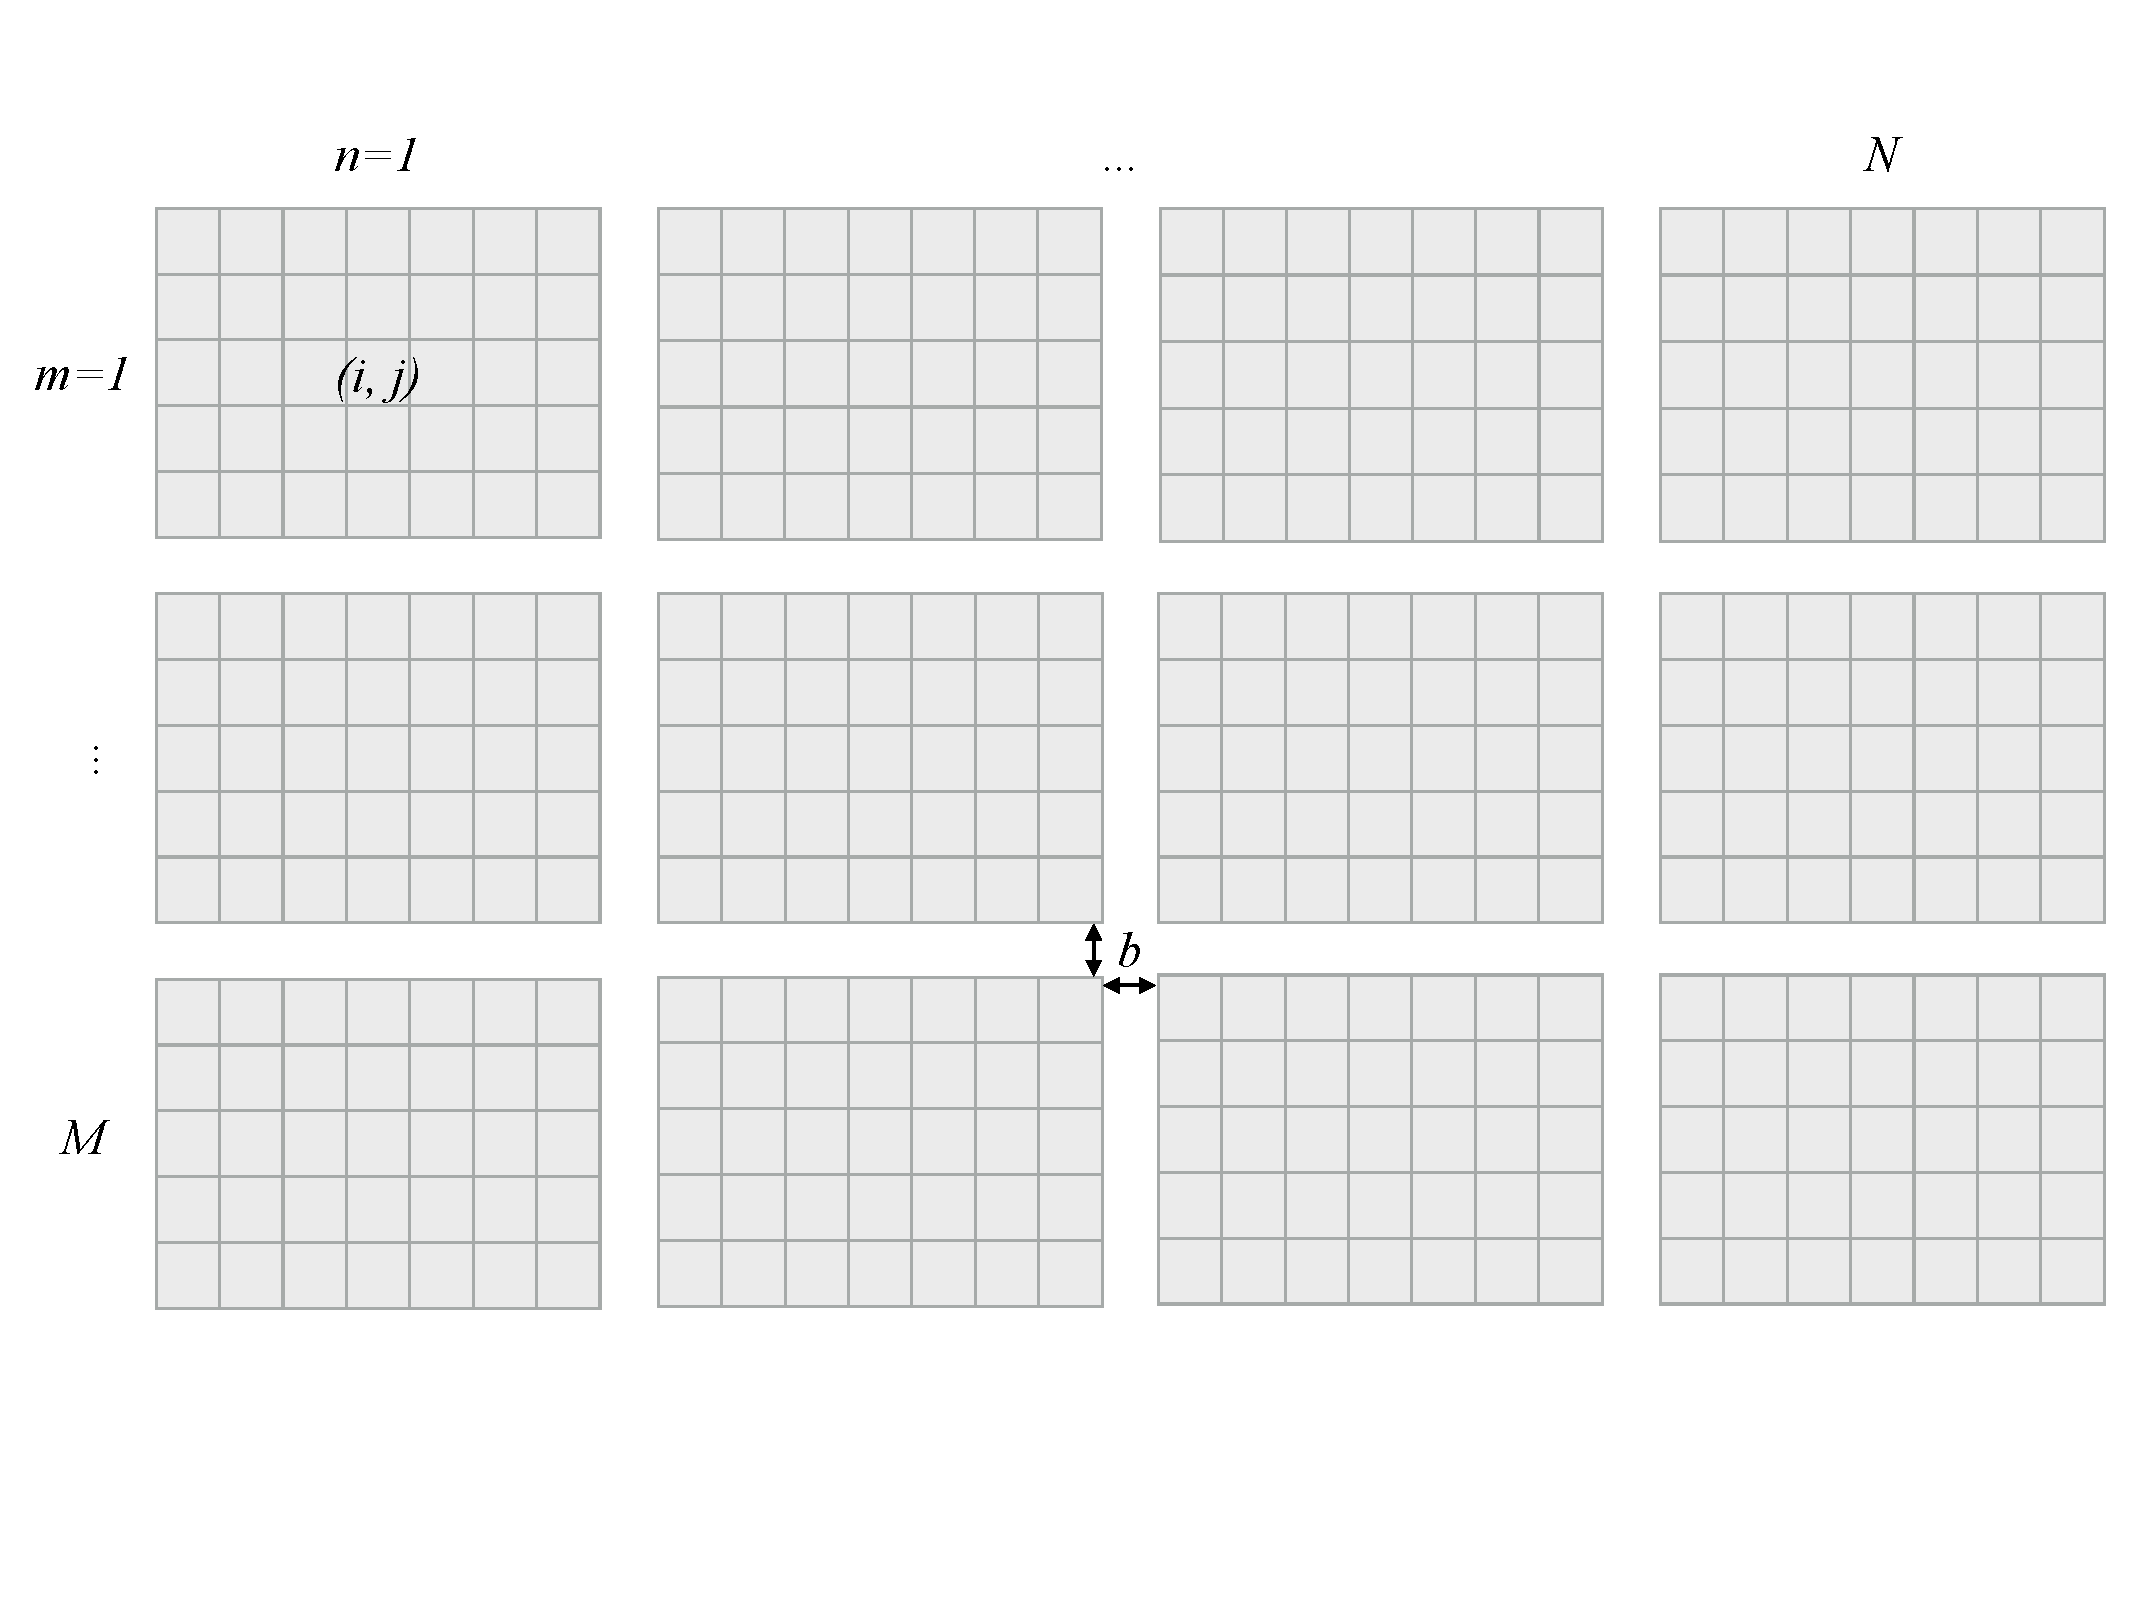
\includegraphics[width=360pt,height=250pt]{img/year-diagram} 

}

\caption{Illustration of the indexing layout for months of one year, where \(M\) and \(N\) indicate number of rows and columns, \(b\) is a space parameter separating cells.}\label{fig:year-diagram}
\end{figure}



Each cell forms a canvas on which to draw the data. Initialize the canvas to have limits \([0, 1]\) both horizontally and vertically. For the pedestrian sensor data, within each cell, hour is plotted horizontally and count is plotted vertically. Each variable is scaled to have values in \([0, 1]\), using the minimum and maximum of all the data values to be displayed, assuming fixed scales. Let \(h\) be the scaled hour, and \(c\) the scaled count.

Then the final points for making the calendar line plots of the pedestrian sensor data is given by:

\begin{equation}
  \begin{aligned}
  x &= j + (n - 1) \times 7 + (n - 1) \times b + h, \\
  y &= i - (m - 1) \times 5 - (m - 1) \times b + c.
  \end{aligned}
  \label{eq:final}
\end{equation}

Note that for the vertical direction, the top left is the starting point of the grid (in Figure \ref{fig:month-diagram}) which is why subtraction is performed. Within each cell, the starting position is the bottom left.

\begin{figure}

{\centering 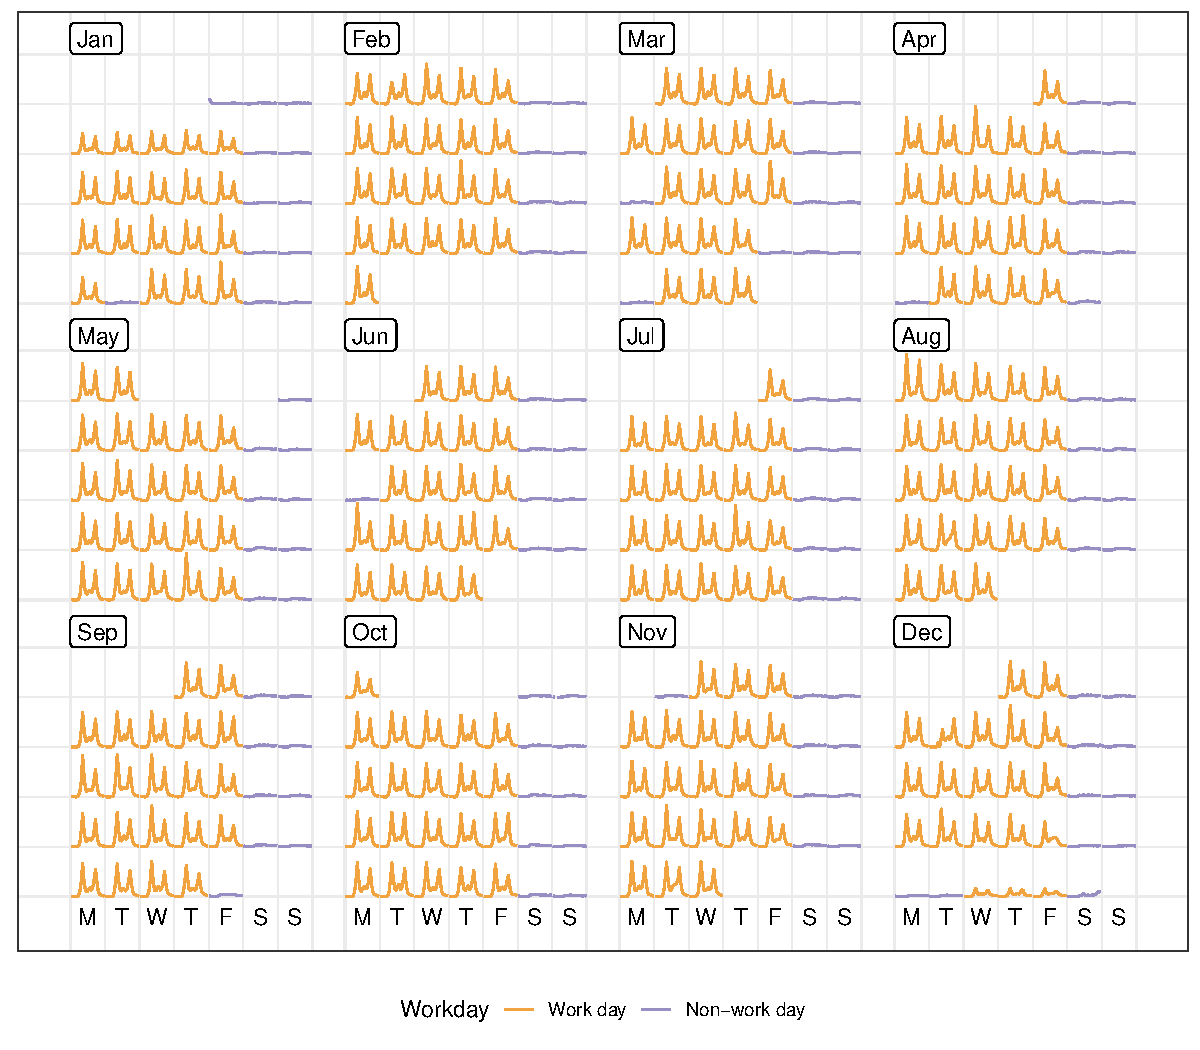
\includegraphics[width=\textwidth]{figure/fs-2016-1} 

}

\caption{The calendar-based display of hourly foot traffic at Flagstaff Station using line glyphs. The disparities between week day and weekend along with public holiday are immediately apparent. The arrangement of the data into a \(3 \times 4\) monthly grid represents all the traffic in 2016. Note that the algorithm wraps the last few days in the sixth week to the top row of each month block for a compact layout, which occurs to May and October.}\label{fig:fs-2016}
\end{figure}



Figure \ref{fig:fs-2016} shows the line glyphs framed in the monthly calendar over the year 2016. This is achieved by the \texttt{frame\_calendar} function, which computes the coordinates on the calendar for the input data variables. These can then be plotted using the usual \textbf{ggplot2} R package \citep{R-ggplot2} functions. All of the grammar of graphics can be applied.

In order to make calendar-based graphics more accessible and informative, reference lines dividing each cell and block as well as labels indicating week day and month are also computed before plot construction.

Regarding the monthly calendar, the major reference lines separate every month panel and the minor ones separate every cell, represented by the thick and thin lines in Figure \ref{fig:fs-2016}, respectively. The major reference lines are placed surrounding every month block: for each \(m\), the vertical lines are determined by \(\min{(x)}\) and \(\max{(x)}\); for each \(n\), the horizontal lines are given by \(\min{(y)}\) and \(\max{(y)}\). The minor reference lines are only placed on the left side of every cell: for each \(i\), the vertical division is \(\min{(x)}\); for each \(j\), the horizontal is \(\min{(y)}\).

The month labels located on the top left using \((\min{(x)}, \max{(y)})\) for every \((m, n)\). The week day texts are uniformly positioned on the bottom of the whole canvas, that is \(\min{(y)}\), with the central position of a cell \(x / 2\) for each \(j\).

\hypertarget{sec:opt}{%
\subsection{Options}\label{sec:opt}}

The algorithm has several optional parameters that modify the layout, direction of display, scales, plot size and switching to polar coordinates. These are accessible to the user by the inputs to the function \texttt{frame\_calendar}:

\begin{verbatim}
frame_calendar(data, x, y, date, calendar = "monthly", dir = "h", 
  week_start = 1, nrow = NULL, ncol = NULL, polar = FALSE, scale = "fixed", 
  width = 0.95, height = 0.95, margin = NULL)
\end{verbatim}

It is assumed that the \texttt{data} is in tidy format \citep{wickham2014tidy}, and \texttt{x}, \texttt{y} are the variables that will be mapped to the horizontal and vertical axes in each cell. For example, the \texttt{x} is the time of the day, and \texttt{y} is the count (Figure \ref{fig:fs-2016}). The \texttt{date} argument specifies the date variable used to construct the calendar layout.

The algorithm handles displaying a single month or several years. The arguments \texttt{nrow} and \texttt{ncol} specify the layout of multiple months. For some time frames, some arrangements may be more beneficial than others. For example, to display data for three years, setting \texttt{nrow\ =\ 3} and \texttt{ncol\ =\ 12} would show each year on a single row.

\hypertarget{layouts}{%
\subsubsection{Layouts}\label{layouts}}

The monthly calendar is the default, but two other formats, weekly and daily, are available with the \texttt{calendar} argument. The daily calendar arranges days along a row, one row per month. The weekly calendar stacks weeks of the year vertically, one row for each week, and one column for each day. The reader can scan down all the Mondays of the year, for example. The daily layout puts more emphasis on day of the month. The weekly calendar is appropriate if most of the variation can be characterized by days of the week. On the other hand, the daily calendar should be used when there is a yearly effect but not a weekly effect in the data (for example weather data). When both effects are present, the monthly calendar would be a better choice. Temporal patterns motivate which variant should be employed.

\hypertarget{orientation}{%
\subsubsection{Orientation}\label{orientation}}

By default, grids are laid out horizontally. This can be transposed by setting the \texttt{dir} parameter to \texttt{"v"}, in which case \(i\) and \(j\) are swapped in Equation \eqref{eq:grid}. This can be useful for creating calendar layouts for countries where vertical layout is the convention.

\hypertarget{start-of-the-week}{%
\subsubsection{Start of the week}\label{start-of-the-week}}

The start of the week for a monthly calendar is adjustable. The default is Monday (\texttt{1}), which is chosen from the data perspective. The week, however, can begin with Sunday (\texttt{7}) as commonly used in the US and Canada, or other week day subject to different countries and cultures.

\hypertarget{polar-transformation}{%
\subsubsection{Polar transformation}\label{polar-transformation}}

When \texttt{polar\ =\ TRUE}, a polar transformation is carried out on the data. The computation is similar to the one described in \citet{Wickham2012glyph}. The resulting plot is star glyphs embedded in the monthly calendar layout. Star glyphs are time series lines transformed in polar coordinates.



\hypertarget{scales}{%
\subsubsection{Scales}\label{scales}}

By default, global scaling is done for values in each plot, with the global minimum and maximum used to fit values into each cell. If the emphasis is comparing trend rather than magnitude, it is useful to scale locally. For temporal data this would harness the temporal components. The choices include: free scale within each cell (\texttt{free}), cells derived from the same day of the week (\texttt{free\_wday}), or cells from the same day of the month (\texttt{free\_mday}). The scaling allows for the comparisons of absolute or relative values, and the emphasis of different temporal variations.

With local scaling, the overall variation gives way to the individual shape. Figure \ref{fig:fs-free} shows the same data as Figure \ref{fig:fs-2016} scaled locally using \texttt{scale\ =\ "free"}. The daily trends are magnified.

\begin{figure}

{\centering 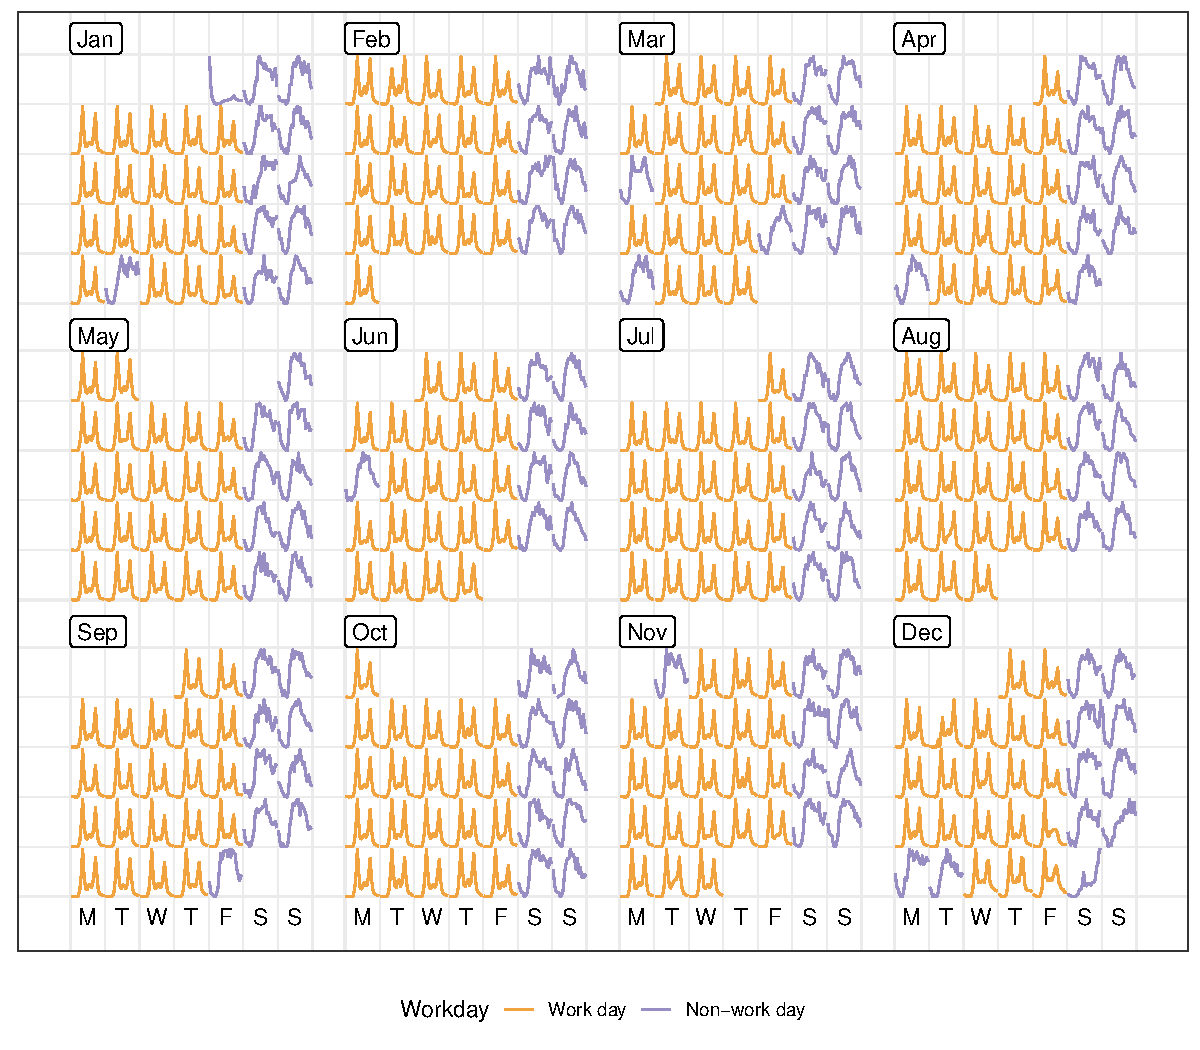
\includegraphics[width=\textwidth]{figure/fs-free-1} 

}

\caption{Line glyphs on the calendar format showing hourly foot traffic at Flagstaff Station, scaled over all the days. The individual shape on a single day becomes more distinctive, however it is impossible to compare the size of peaks between days.}\label{fig:fs-free}
\end{figure}



The \texttt{free\_wday} scales each week day together. It can be useful to comparing trends across week days, allowing relative patterns for weekends versus week days to be examined. Similarly, the \texttt{free\_mday} uses free scaling for any day within a given month.

\hypertarget{language-support}{%
\subsubsection{Language support}\label{language-support}}

Most countries have adopted this western calendar layout, while the languages used for week day and month would be different across countries. We also offer language specifications other than English for text labelling.

\hypertarget{sec:variations}{%
\subsection{Variations}\label{sec:variations}}

\hypertarget{overlaying-and-faceting-subsets}{%
\subsubsection{Overlaying and faceting subsets}\label{overlaying-and-faceting-subsets}}

Plots can be layered. The comparison of sensors can be done by overlaying the values for each (Figure \ref{fig:overlay}). Differences between the pedestrian patterns at these sensors can be seen. Flagstaff Station exhibits strong commuters patterns, with fewer pedestrian counts during the weekends and public holidays. This suggests that Flagstaff Station has limited functionality on non-work days. From Figure \ref{fig:overlay} it can be seen that Birrarung Marr has a distinct temporal pattern from the other two all year round. The nighttime events, such as White Night, have barely affected the operation of Flagstaff Station but heavily affected the incoming and outgoing traffic to the State Library and Birrarung Marr.

\begin{figure}

{\centering 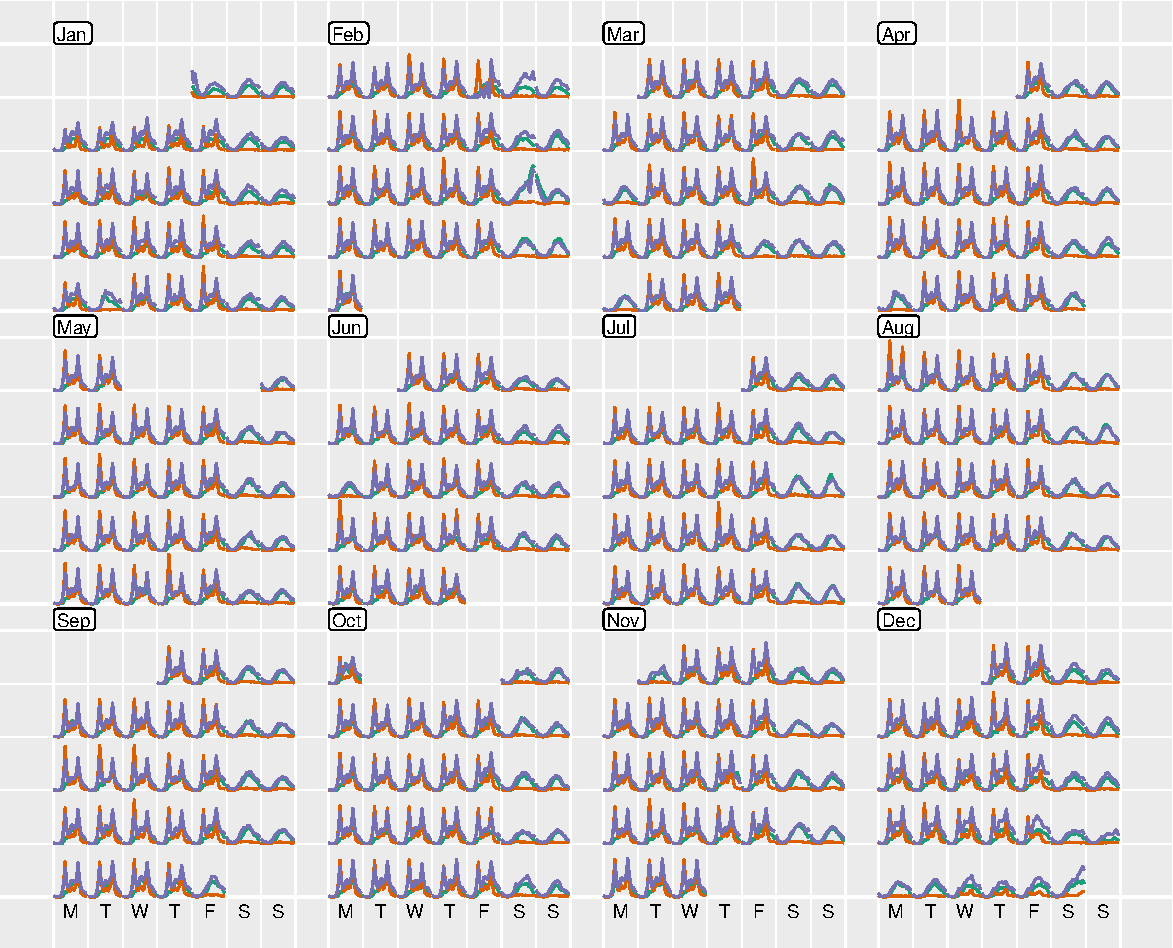
\includegraphics[width=\textwidth]{figure/overlay-1} 

}

\caption{Overlaying line graphs of the three sensors in the monthly calendar. Three sensors demonstrate very different traffic patterns. Birrarung Marr tends to attract many pedestrians for special events held on weekends, contrasting to the bimodal commuting traffic at Flagstaff Station.}\label{fig:overlay}
\end{figure}



To avoid the overlapping problem, the calendar layout can be embedded into a series of subplots for the different sensors. Figure \ref{fig:facet} presents the idea of faceting calendar plots. This allows comparing the overall structure between sensors, while emphasizing individual sensor variation. In particular, it can be immediately learned that Birrarung Marr was busy and packed, for example during the Australian Open, a major international tennis tournament, in the last two weeks of January. This is concealed in the conventional graphics.

\begin{figure}

{\centering 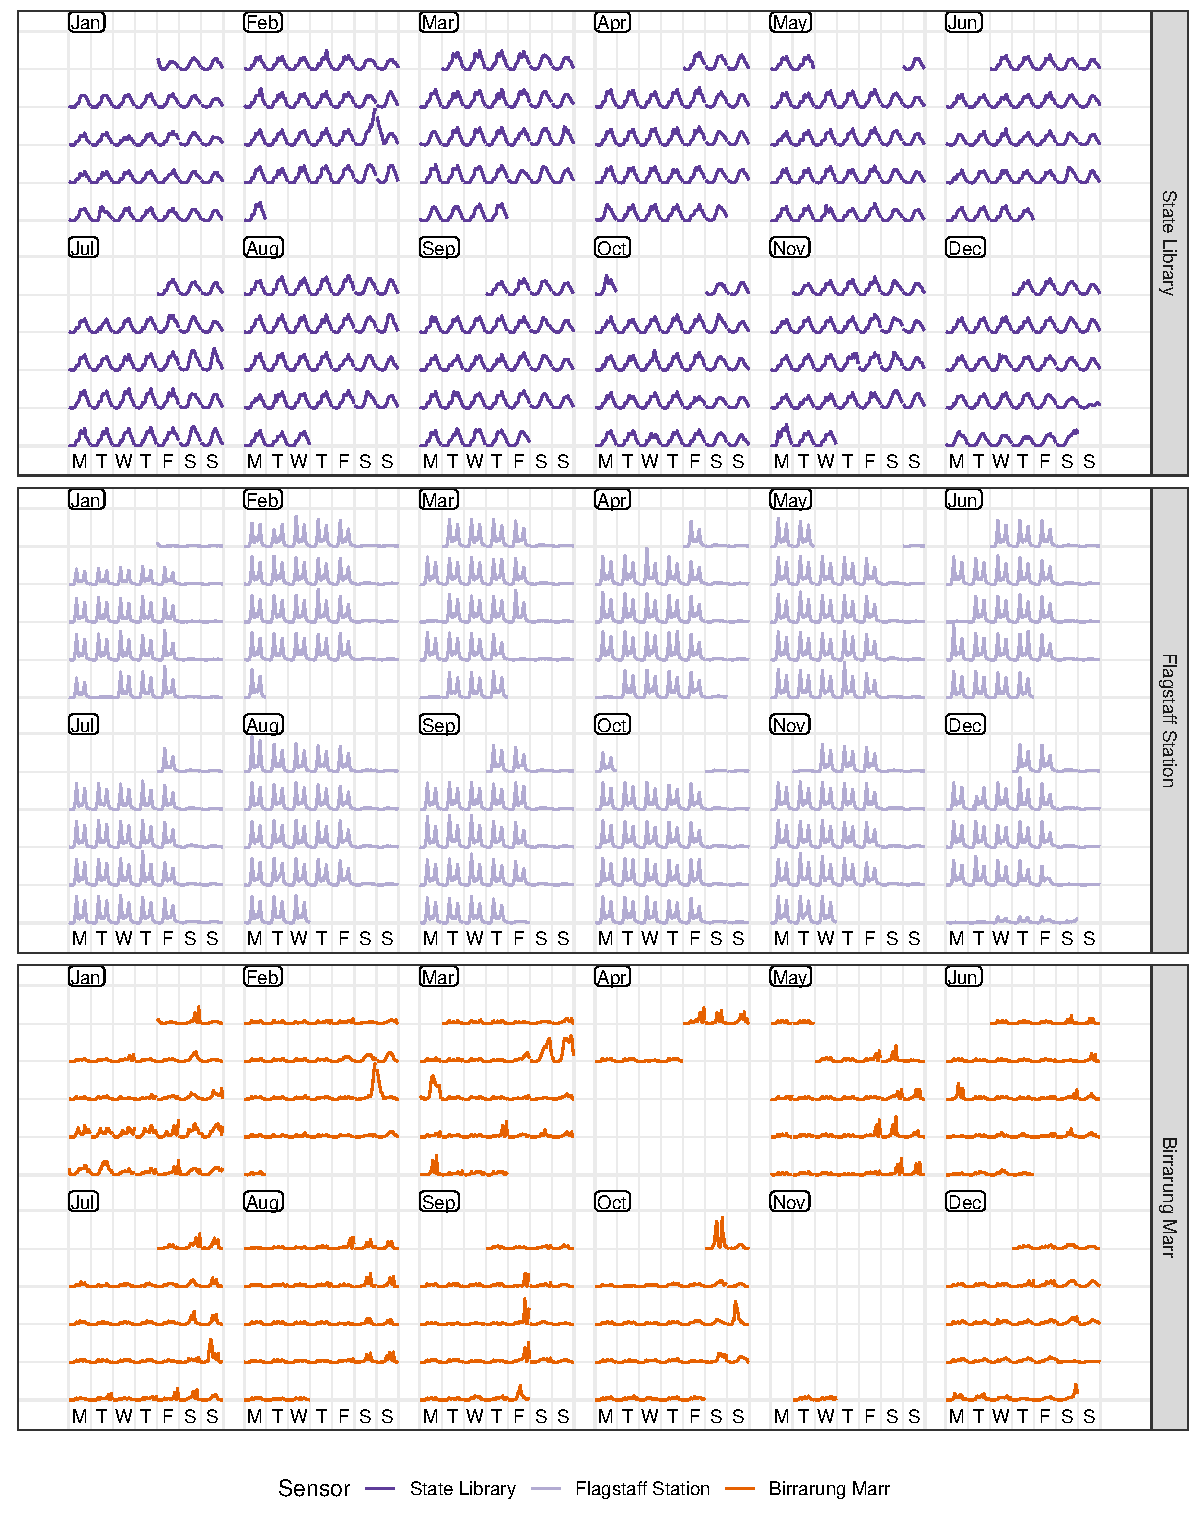
\includegraphics[width=\textwidth]{figure/facet-1} 

}

\caption{Line charts, embedded in the \(6 \times 2\) monthly calendar, colored and faceted by the 3 sensors. The variations of an individual sensor are emphasised, and the shapes can be compared across the cells and sensors.}\label{fig:facet}
\end{figure}



\hypertarget{different-types-of-plots}{%
\subsubsection{Different types of plots}\label{different-types-of-plots}}

The \texttt{frame\_calendar} function is not constrained to line plots. The full range of plotting capabilities in \textbf{ggplot2} is essentially available. Figure \ref{fig:scatterplot} shows a lag scatterplot with local scaling for each day at Flagstaff Station, where the lagged hourly count is assigned to the \texttt{x} argument and the current hourly count to the \texttt{y} argument. This figure is organized in the daily calendar layout. Figure \ref{fig:scatterplot} indicates two dominate patterns, strong autocorrelation on weekends, and weaker autocorrelation on work days. At the higher counts on week days, the next hour sees possibly substantial increase or decrease in counts, as is depicted as the V-shape in the graphs. This is consistent with the bimodality from Figure \ref{fig:fs-2016}, since positive correlations are perceived when approaching to the peak hour yet negative correlations when moving away from the peak hour.

\begin{figure}

{\centering 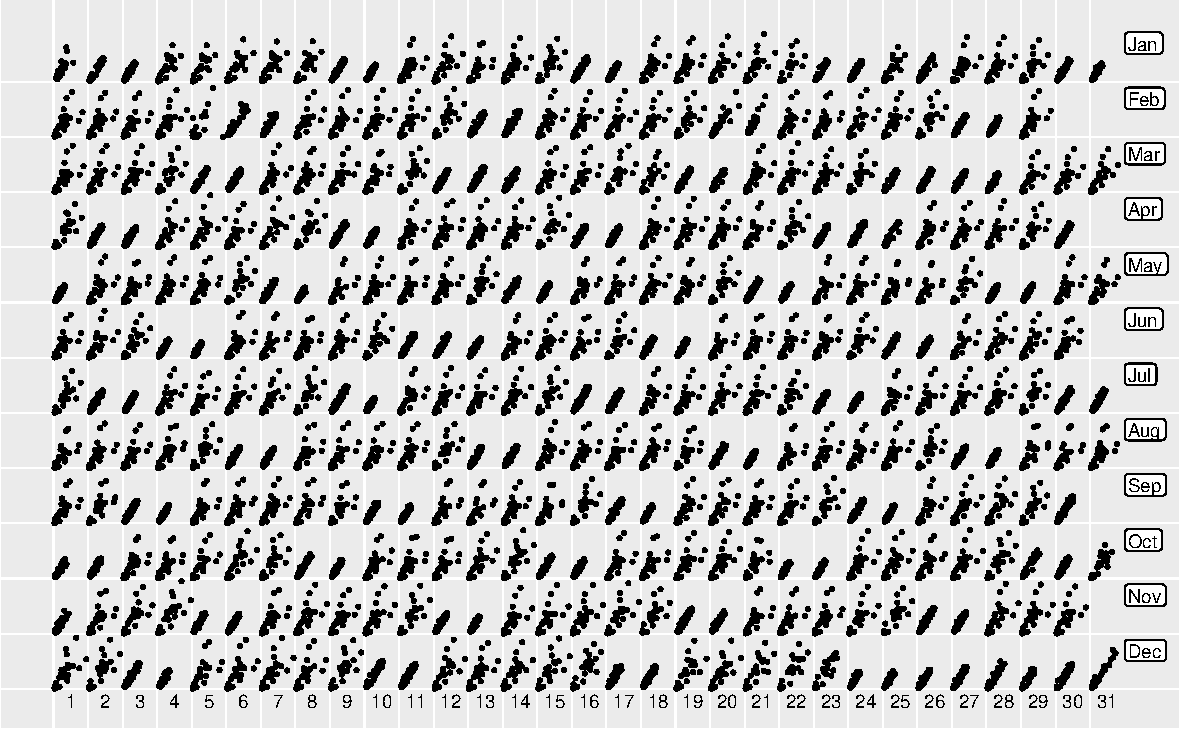
\includegraphics[width=\textwidth]{figure/scatterplot-1} 

}

\caption{Lag scatterplot with local scaling in the daily calendar layout. Each hour's count is plotted against previous hour's count at Flagstaff Station to demonstrate the autocorrelation at lag 1. The correlation between them is more consistent on non-work days than work days.}\label{fig:scatterplot}
\end{figure}



The algorithm can also produce more complicated plots, such as boxplots. Figure \ref{fig:boxplot} uses a loess smooth line \citep{cleveland1979loess} superimposed on side-by-side boxplots. It shows the distribution of hourly counts across all 43 sensors during December. The last week of December is the holiday season: people are off work on the day before Christmas (December 24), go shopping on the Boxing day (December 26), and stay out for the fireworks on New Year's Eve.

\begin{figure}

{\centering 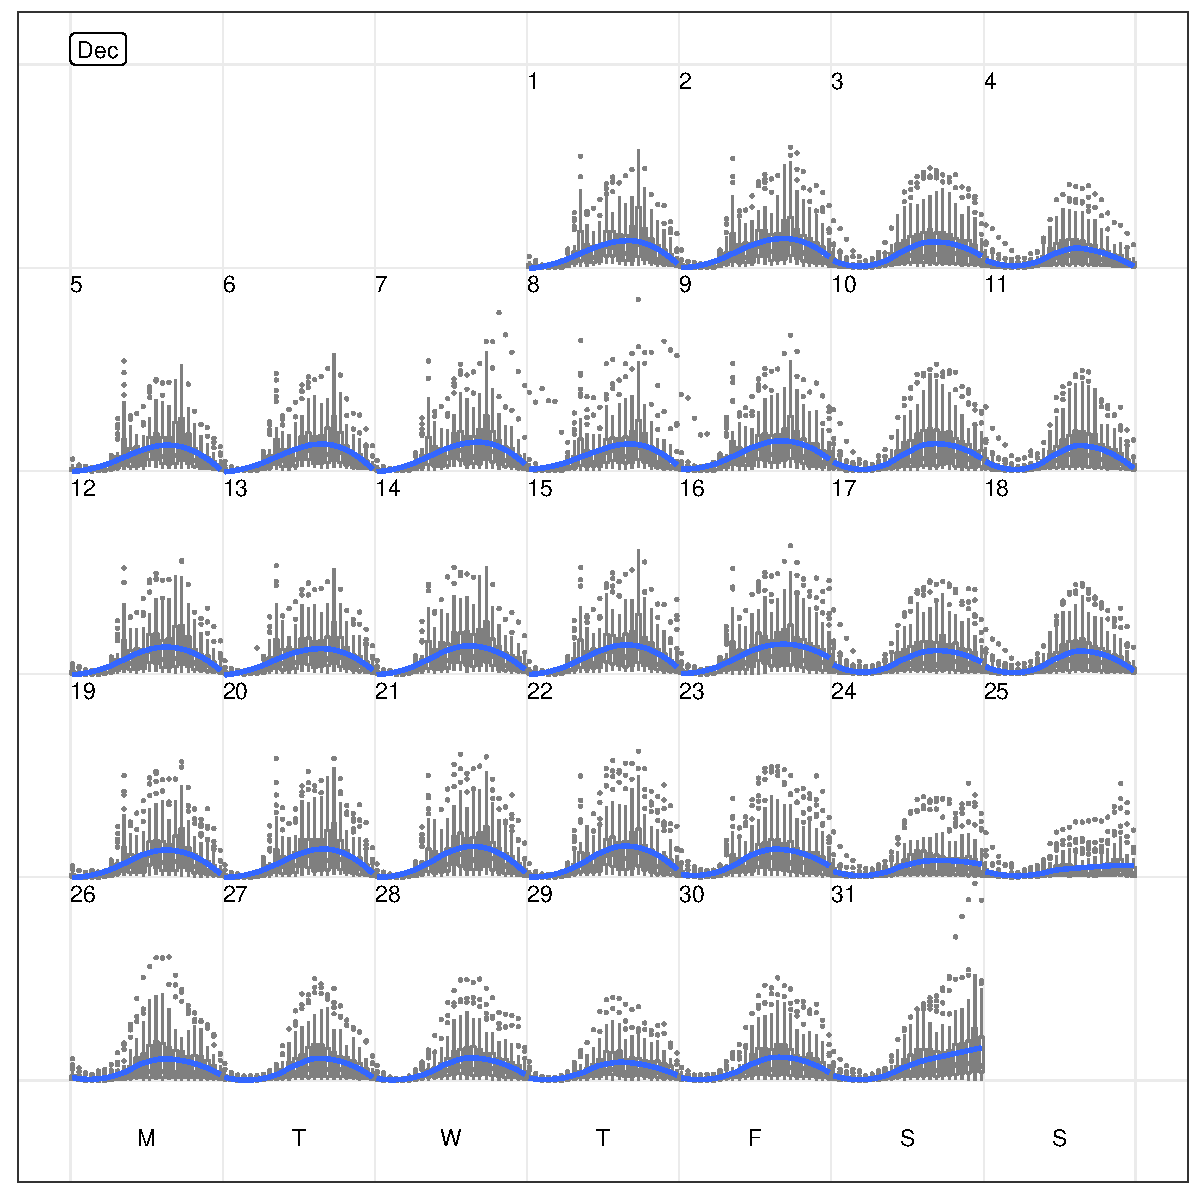
\includegraphics[width=\textwidth]{figure/boxplot-1} 

}

\caption{Side-by-side boxplots of hourly counts for all the 43 sensors in December 2016, with the loess smooth line superimposed on each day. It shows the hourly distribution in the city as a whole. The increased varibility is noted on the last day of December as approaching towards New Year's Eve.}\label{fig:boxplot}
\end{figure}

\begin{figure}

{\centering 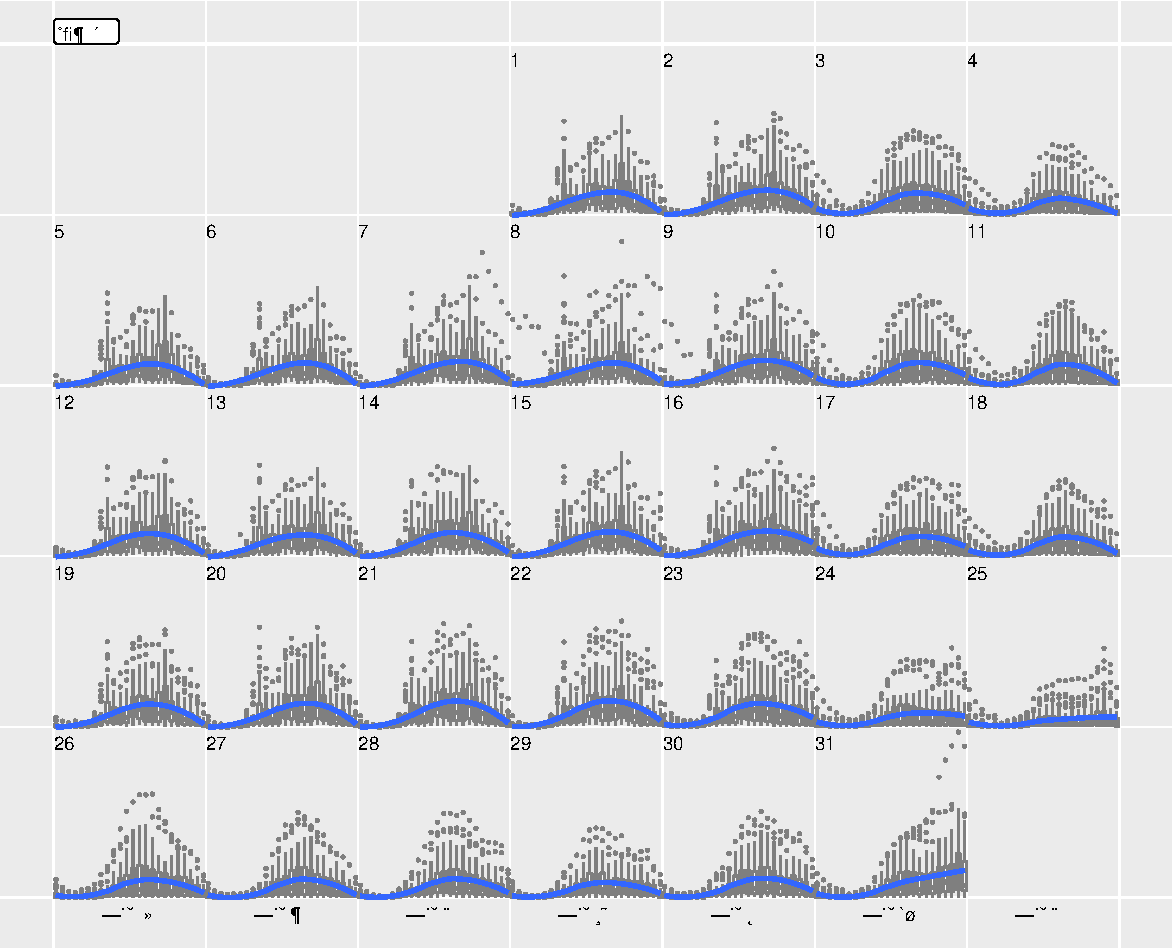
\includegraphics[width=\textwidth]{figure/chn-1} 

}

\caption{The same plot as Figure \ref{fig:boxplot}, but with the month and week day labels in Chinese. It demonstrates the natural support for languages other than English.}\label{fig:chn}
\end{figure}



\hypertarget{interactivity}{%
\subsubsection{Interactivity}\label{interactivity}}

As a data restructuring tool, the interactivity of calendar-based displays can be easily enabled, as long as the interactive graphic system remains true to the spirit of the grammar of graphics, for example \textbf{plotly} \citep{plotly} in R. As a standalone display, an interactive tooltip can be added to show labels when mousing over it in the calendar layout, for example the hourly count with the time of day. It is difficult to sense the values from the static display, but the tooltip makes it possible. Options in the \texttt{frame\_calendar} function can be ported to a form of selection button or text input in a graphical user interface like R shiny \citep{R-shiny}. The display will update on the fly accordingly via clicking or text input, as desired.

Linking calendar displays to other types of charts is valuable to visually explore the relationships between variables. An example can be found in the \textbf{wanderer4melb} shiny application \citep{R-wanderer4melb}. The calendar most naturally serves as a tool for date selection: by selecting and brushing the glyphs in the calendar, it subsequently highlights the elements of corresponding dates in other time-based plots. Conversely, selecting on weather data plots, linked to the calendar can help to assess if very hot/cold days and heavy rain affect the number of people walking in downtown Melbourne. The linking between weather data and calendar display is achieved using the common dates.

\hypertarget{reasons-to-use-calendar-based-graphics}{%
\subsection{Reasons to use calendar-based graphics}\label{reasons-to-use-calendar-based-graphics}}

The calendar-based graphics provides a contextual canvas to plot glyphs into a familiar calendar format. The purpose of this calendar display is to facilitate quick discoveries of unusual patterns in people's activities, which is critical in data visualisation. It not only complements the traditional graphical toolbox for understanding general trends, but it profiles vivid and detailed data stories about the way we live. Comparing to Figure \ref{fig:time-series-plot} and \ref{fig:facet-time}, Figure \ref{fig:facet} is more informatively compelling: whether special events happened on which day and whether they are day or night events. Figure \ref{fig:facet} informs that many events were held in Birrarung Marr during weekends, while September's events took place on Fridays, which is difficult to discern in the other two plots.

\hypertarget{sec:facet-calendar}{%
\section{A fully-fledged faceting calendar method}\label{sec:facet-calendar}}

\begin{center}\includegraphics[width=\textwidth]{figure/facet-calendar-1} \end{center}

\hypertarget{sec:case}{%
\section{Case study}\label{sec:case}}

The use of the calendar display is illustrated on smart meter energy usage from four households in Melbourne, Australia. Individuals can download their own data from the energy supplier, and the data contained in the paper is made available from four colleagues of the authors. The calendar display is useful to help people understand their energy use. The data contains half-hourly electricity consumption in the first half of 2018. The analysis begins by looking at the distribution over days of week, then time of day split by work days and non-work days, followed by the calendar display to inspect the daily schedules.

Figure \ref{fig:dow} shows the energy use across days of week in the form of letter value plots \citep{hofmann2017letter}. Letter value plots are a variant of boxplots for large data, with other quantiles represented by boxes. Letters indicate the fraction of the data divisions, for example, F indicates fourths or quartiles, and the two outer ends of the box are the 25th and 75th percentile, the same traditional ends of the box as a boxplot. The letter E indicates eighths, with box ends being 12.5th and 87.5th percentiles of the data. These additional boxes replace the whiskers in a traditional boxplot. The letter value plots for the households, show a line indicating the median (M) and the innermost boxes corresponding to the fourth (F) and the eighth (E) quantile divisions. Inspecting the medians across households tells us that household 3, a family size of one couple and two kids, uses more energy over the week days, than other households. The relatively larger boxes for household 2 indicates greater variability in daily energy consumption with noticeable variations on Thursdays, and much higher usage over the weekends. The other two households (1 and 4) tend to consume more energy with more variation on the weekends relative to the week days, reflecting of work and leisure patterns.

\begin{figure}

{\centering 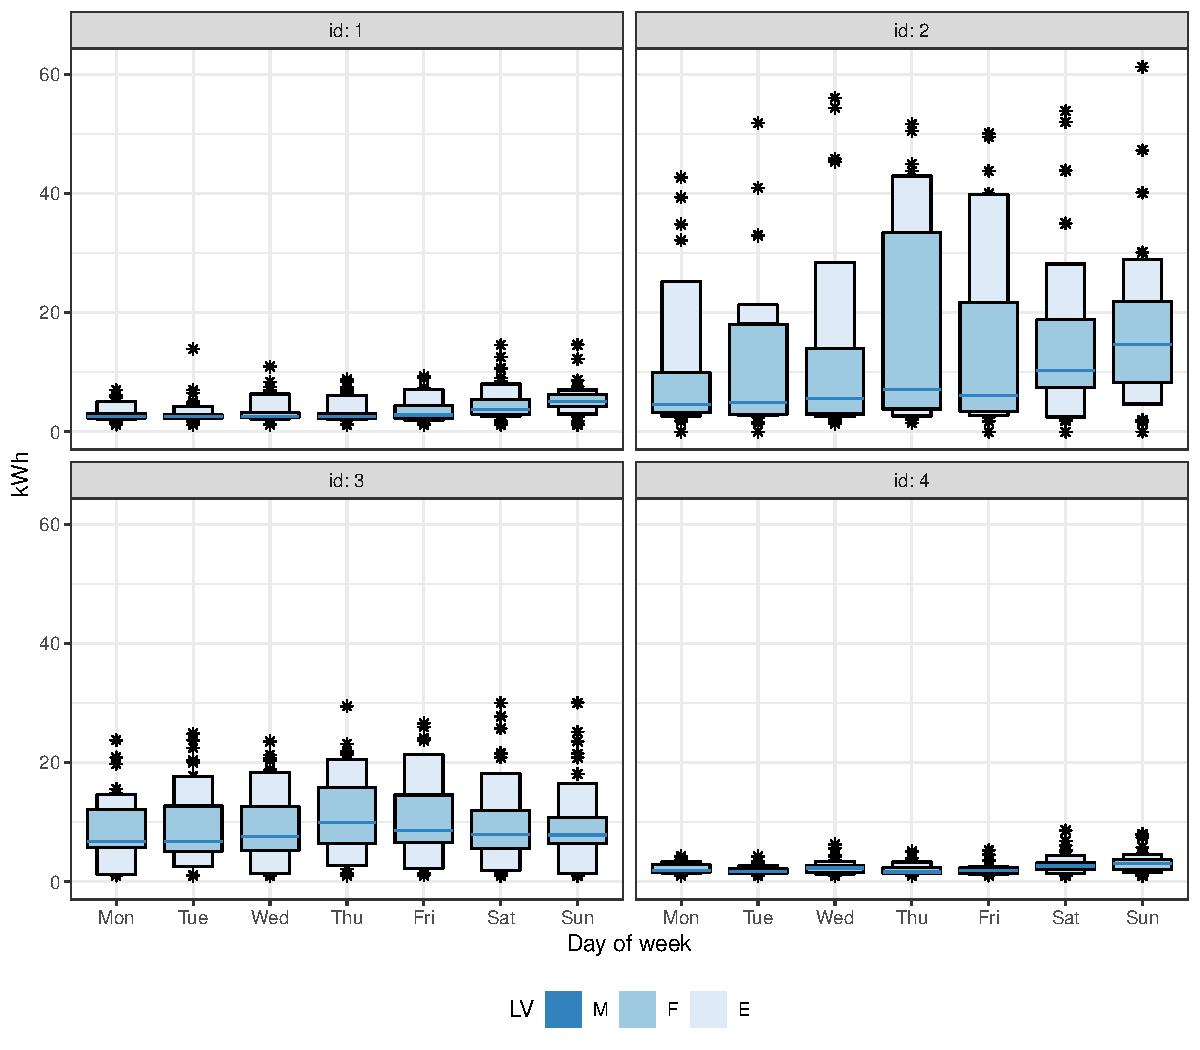
\includegraphics[width=\textwidth]{figure/dow-1} 

}

\caption{Letter value plots of daily energy usage against day of week for four households, with one line dislaying the median (M) and each box corresponding to the fourth (F) and eighth (E) paired quantile estimates. Suggested by the medians, household 3 uses more enery than the others on the week days, due to a large family size. By constrast, household 2 sees considerally large variability.}\label{fig:dow}
\end{figure}

Figure \ref{fig:hod} shows energy consumption against time of day, separately by week day and weekend. Household 1 is an early bird, starting their day before 6 and going back home around 18 on week days. They switch air conditioning on when they get home from work and keep it operating until mid-night, learned from the small horizontal cluster of points around 0.8 kWh. On the other hand, the stripes above 1 kWh for household 2 indicates that perhaps air conditioning runs continuously for some periods, consuming the twice the energy as household 1. A third peak occurs around 15 for household 3 only, likely when the kids are home from school. They also have a consistent energy pattern between week days and weekends. As for household 4, their home routine starts after 18 on week days. Figures \ref{fig:dow} and \ref{fig:hod}, part of a traditional graphical toolkit, are useful for summarizing overall deviations across days and households.

\begin{figure}

{\centering 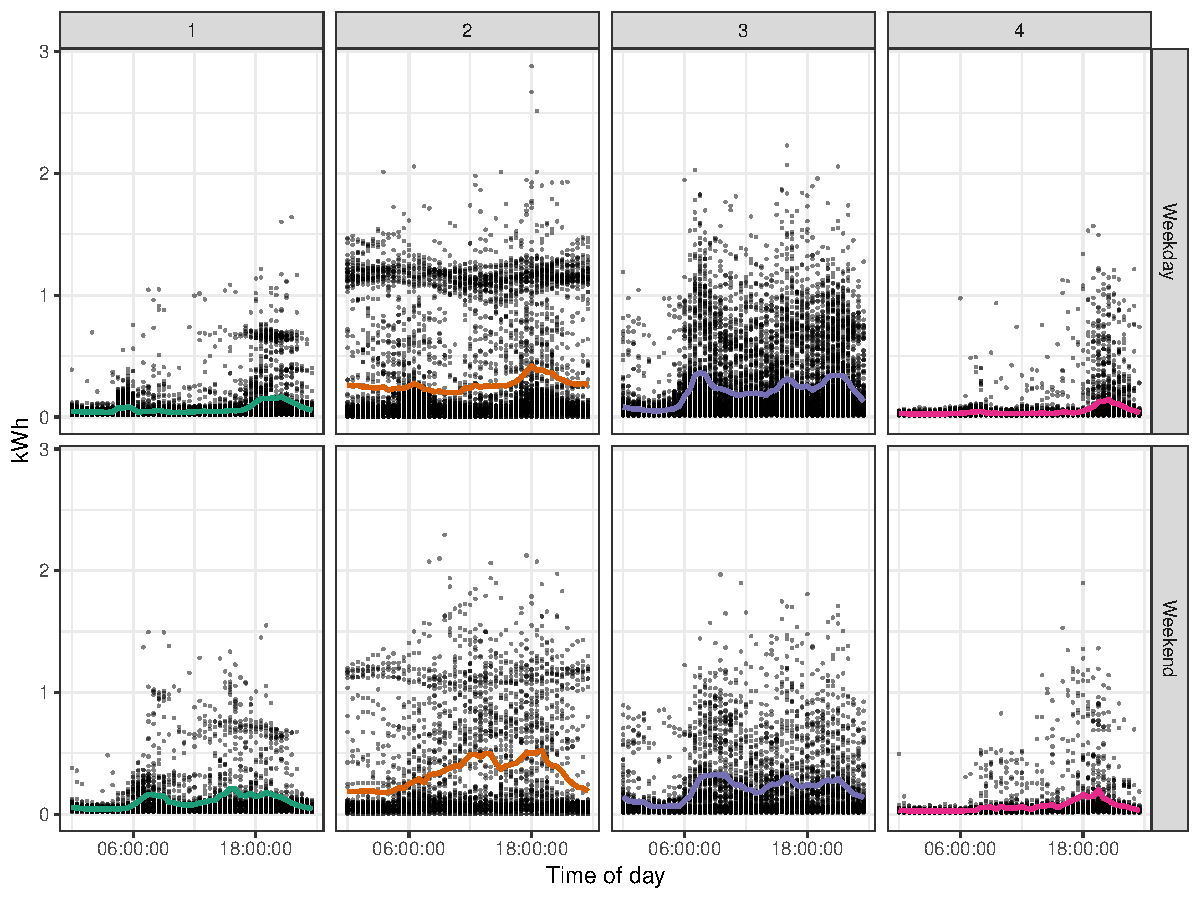
\includegraphics[width=\textwidth]{figure/hod-1} 

}

\caption{Scatterplot between half-hourly energy usage and time of day with the averages overlaid, constrasting week days and weekends for each household. All have different daily routines between week days and weekends, except for household 3. On week days, household 1 wakes up early before 6, and household 2 around 6, followed by household 3 and 4. The use of air conditioning is noted in household 1 and 2.}\label{fig:hod}
\end{figure}

Figure \ref{fig:calendar-elec} displays the global scaling of each household's data in calendar layout, unfolding their day-to-day life via electricity usage. Glancing over household 1, we can see that their overall energy use is relatively low. Their week day energy use is distinguishable from their weekends, indicating a working household. The air conditioner appears to be used in the summer months (January and February) for a couple of hours in the evening and weekends. In contrast, household 2 keeps cooling system functioning for much longer hours, which becomes more evident from late Wednesday through Thursday to early Friday in the mid January. These observations help to explain the stripes and clusters of household 2 in Figure \ref{fig:hod}. It is difficult to give a succinct description of household 3 since everyday energy pattern is variable, but May and June see more structures than the previous months. Individual data can be idiosyncratic, hence aggregated plots like Figure \ref{fig:dow} and \ref{fig:hod} are essential for assembling pieces to pictures. However, the calendar plots speak the stories about the exact vacation time that are untold by previous plots, for example their vacation time. Household 1 is on vacation over three weeks of mid June, and household 2 also planned to take some days off in the second week of June. Further household 3 takes one short trip in January and the other one starting in the fourth week of June. Household 4 is away over two or three weeks early April and late June. They all tend to take breaks during June due to the fact that the University winter break starts in June.

\begin{figure}

{\centering \includegraphics[width=\textwidth]{figure/calendar-elec-1} 

}

\caption{Calendar displays for each household using common scales. We can precisely tell each indidual's vacation days to take off and the overnight use for household 2.}\label{fig:calendar-elec}
\end{figure}

\hypertarget{sec:discussion}{%
\section{Discussion}\label{sec:discussion}}

The calendar-based visualization provides data plots in the familiar format of an everyday tool. Patterns on special events and public holidays for the region are more visible to the viewer.

The methodology creates the western calendar layout, because most countries have adopted this format. The main difference between countries is the use of different languages for labeling, which is supported by the software. Layouts beyond the western calendar could be achieved by the same modular arithmetic approach.

The calendar layout will be useful for studying consumer trends and human behavior. It will not be so useful for physical patterns like climate, which are not typically affected by human activity. The layout does not replace traditional displays, but serves to complement to further tease out structure in temporal data. Analysts would still be advised to plot overall summaries and deviations in order to study general trends.

\hypertarget{acknowledgements}{%
\section*{Acknowledgements}\label{acknowledgements}}
\addcontentsline{toc}{section}{Acknowledgements}

We would like to thank Stuart Lee and Heike Hofmann for their feedback about this work. The most recent version of the \texttt{frame\_calendar} function is included in the \textbf{sugrrants} R package, which can be accessed via the CRAN website \url{https://CRAN.R-project.org/package=sugrrants} or Github \url{https://github.com/earowang/sugrrants}. All materials required to reproduce this article and a history of the changes can be found at the project's Github repository \url{https://github.com/earowang/paper-calendar-vis}.

\bibliographystyle{agsm}
\bibliography{bibliography.bib}

\end{document}
